\documentclass[12pt,a4paper]{article}
\usepackage{times}
\usepackage{durhampaper}

\usepackage{harvard}
% package to add dumptext
\usepackage[english]{babel}
\usepackage{blindtext}

% packages to add images
\usepackage{graphicx}

% packages for pseudocode and algorithms
\usepackage{amsmath}
\usepackage{algorithm}
\usepackage[noend]{algpseudocode}
\makeatletter
\def\BState{\State\hskip-\ALG@thistlm}
\makeatother

% packages to generate neural network graph
\usepackage{tikz}
\usetikzlibrary{positioning}

% package to add graphs
\usepackage{pgfplots}

\citationmode{abbr}
\bibliographystyle{agsm}

\title{Improving CNN Draughts Evaluators using Genetic Algorithms}
\author{Thien P. Nguyen}
\student{Thien P. Nguyen}
\supervisor{Stefan Dantchev}
\degree{BSc Computer Science}

\date{}

\begin{document}

\maketitle

\begin{abstract}

{\bf Background}

Presently, competitive Draughts AI players are currently designed to play at a fixed ability. While it has produced very competitive and intelligent players, they require manual modifications in order to improve its performance. This is due to their dependency on pre-defined move databases, where optimal moves are pre-calculated, and recalled when necessary. By combining Neural Networks and Genetic Algorithms, this issue could possibly be solved by creating a player that can grow in ability over time, without the dependency on move-banks.
 
{\bf Aims}

 The purpose of this project is to explore approaches to tackle the game of English Draughts via the use of  machine learning techniques. First, we study previous historical successes in the field, and look at the components that helped build their systems. Then, we look at contemporary methods of computer science that could be used to evolve the historical systems. The project will establish whether this approach provides an effective performance on the game.
 
{\bf Method}

The initial population will consist of randomly generated AI players, which will play each other to determine the best player out of the population. The performance of championing AI players at every generation of the genetic algorithm are measured against previous champions. Appropiate algorithms are implemented to detect the overall development of the system's ability to play Checkers.

{\bf Proposed Solution}.  

The proposed solution starts with designing a neural network that evaluates the probability of a particular side winning, given a given state of a checkerboard. This is then used in a algorithm that evaluates future moves to predict the best move at a given position. This, alongside a set of weights for the neural network, creates a player that can evaluate potential moves. Finally, the player is then used on an existing Draughts framework that will provide the player with the ability to play Draughts.

\end{abstract}

\begin{keywords}
AI, Neural Networks, Genetic Algorithms, MiniMax, Alpha Beta Pruning, Draughts

\end{keywords}

% ----------------

% Sort introduction to your project
% This will be the first thing that your second marker sees about your project
% Make sure they can understand what you’re doing
% Write for educated reader with background in CS, but non-expert Should contain:

%   Brief introduction to the project
%   The research question you are addressing
%   Aims of the project 
%   Deliverables


\section{Introduction}
The intention of this project is to explore the effectiveness of genetic algorithms to improve the evaluation of a neural network's probability to determine the performance of two players in a game of checkers. We attempt to use various crossover and mutation strategies to manipulate the weights of the network, and compare their performance relative to the overall performance of the system.

\subsection*{Draughts}

English Draughts (or Checkers) is a popular 2-player boardgame played on an 8x8 chessboard. Players begin with 12 pieces each, and they are placed on light-coloured squares. Each player takes a turn to move a piece diagonally in one square. They also have the option to capture their opponments piece by moving two consecutive diagonal squares, where the opponments piece is placed immediately opposite the players piece. Pieces can be captured consecutively in a single turn if the moves afford the scenario. In the event that a piece reaches the opposite side of the board from where the piece started with, they are promoted to a 'King' piece. King pieces have the ability to traverse backwards in the same diagonal motion as pawns.

\subsection*{Genetic Algorithms}

Genetic algorithms (GAs) are a group of search techniques used to find exact or approximate solutions to optimisation and search problems. It borrows techniques from Charles Darwin's evolutionism theory; individuals are created by the crossover of the genetic information of their parents. 
Genetic algorithms are a subset of evolutionary algorithms, where the larger group is also formed of similar strategies not including Evolutionary Programming [Fogel, 1993][McDonnel, 1993], and genetic programming [Koza, 1991].

\subsection*{Neural Networks}

Neural Networks are non-linear statistical data-modelling tools, linking inputs and outputs adaptively in a learning process similar to how the human brain operates. Networks consist of units, described as neurons, joined by a set of rules and weights. The units are defined with characterisitics, and appear in layers. The first layer is defined as the input layer, and the last layer being the output. Layers between the two aforementioned are described as hidden layers. Data is analysed by processing them through the layers.

Learning takes place in the form of the manipulation of the weights connecting the units in the layers. This allows it to model complex relationships between inputs and output, and it can also find patterns in the data. 

\subsection*{Motivation}
% Research Question
Whilst the use of evolutionary algorithms and neural networks have been explored to create draughts players, my intention is to explore a subset of evolutionary algorithms to determine their viability. Can we produce a similarly performant draughts evaluator by using seperate classifiers for the different stages of the game? Can the use of genetic algorithms and neural networks (GANNs) make a competent Draughts player?

\subsection*{Deliverables}

\subsubsection*{Minimum}

\begin{itemize}
\item Implement a CNN
\item Implement a Checkers Game Interface
\item Implement a genetic algorithm with an evaluation function that
  consists of a round robin tournament against the population of CNN
  Evaluators.
\item Implement a mini-max algorithm that chooses moves.
\end{itemize}

\subsubsection*{Intermediate}

\begin{itemize}
\item A user-friendly interface to play against the AI
\item A monte-carlo search of the move space.
\item Analysis of Crossover methods (within Genetic Algorithms)
\item Analysis of Mutation methods (within Genetic Algorithms)
\end{itemize}

\subsubsection*{Advanced}

\begin{itemize}
\item Convolutional Neural Network Layer analysis
\item The resulting AI can play to an ELO of at least 1200.
\end{itemize}

\subsection*{Related Work}

% ----------------

\section{Design}

\subsection*{Requirements}

% Functional Requirements
A checkers gameboard is created

Agents are able to select a legal move

Agents are able to harness neural networks to assist in their move decision

Champions are able to create offspring.

The weights and biases of the Agent's neural network are saved to a form of storage.

% Non Functional Requirements
Agents only choose valid, legal moves

Agents always return a valid, legal move

Agents make maximum use of the turn time where appropriate
% Table 1 shows the functional requirements identified for the program(s) that will be required for the project. FR-1 through FR-6 are handled by the server and player implementations in the GGP-Base package. FR-7 will require some modification to the server code in order to output the informationthatwillbeusedintheanalysisanddiscussionoftestingresults.
% Table 2 shows the non-functional requirements that arise from the rules that will be applied for testing. Any failure of the agent to return a move through either error or timeout should be con- sidered a failure as per the AAAI GGP competition rules. The moves returned should always be valid and legal for the current state of the game. Since agents are given a fixed time period to choose a move, with no penalty or bonus applied so long as the move is returned within the allot- ted time, it makes sense that agents should be designed in such a way as to make best use of the time they are given.
% The GGP-Base package addresses a number of these requirements and a number of test-games will be played to ensure they are adequately satisfied and the package functions as expected.
\blindtext

\subsection*{Choice of Programming Language}

The project is to be written in Python 3.6 due to my familiarity, and the support of popular scientific packages including NumPy and other machine learning tools. Python is also portable with a very wide compatability; for instance it is pre-installed on all popular UNIX machines and also has support from the university machines.

Object Oriented approaches are taken for the majority of the components of the system, ranging from the neural network library to the tournament system. Data structures are implemented using their own classes and methods where applicable. 

Players weights (for their neural networks) are stored in two forms, one of which is to be stored on an MongoDB NoSQL instance, and another local copy in JSON. This allows the individual agents to be played against humans.

\subsection*{Tools}

The resulting program will be simulated on Durham's MIRA (128-core Intel) distributed system for 4-ply heavy loads, and debugging will occur on a lighter machine (4-core Intel i5 6200u). In order to keep simulations running on MIRA, MOSH is used to maintain a consistent UDP SSH connection to MIRA. The end champion is then hosted online on a Heroku instance as an API.

\subsection*{Architecture}

Should include a diagram of the algorithm workflow

\blindtext
\blindtext

\subsection*{Algorithms and Data Structures}

% Algorithm 1: Minimax with Monte Carlo Search (MM-MCS)
% This algorithm operates in two phases: the exploration phase and the probe phase. In exploration, the algorithm expands the tree until some fixed depth is reached. During the probe phase, the algorithm repeatedly selects a leaf node with a uniform random probability and explores this by selecting random successor states until a terminal state is reached. The expected value of the fringe node is the total rewards gained from exploring it divided by the number of times it was visited. Figure 5 Illustrates the operation of the algorithm. In this implementation, recursive ex- ploration and probing are performed as two separate stages to enable maximal use ofthe time al- lowed rather than using a fixed number of probes per fringe node. Once a time limit is reached, the algorithm performs a final minimax selection on the tree using values gained from simulation to determine the next move. Algorithm 1 describes the behaviour of MM-MCS.
\subsubsection{Neural Network}

In order to evaluate the board, we use a feed-forward neural network in the form of the following node layers {91,40,10,1} where the input layer consists of 32 nodes, with the output node having 1. Our sigmoidal function of choice is the hyperbolic tangent. The input layer is the board, preprocessed to cover all possible subsquares of the checkerboard, rangig from a 3x3 kernel to a 8x8. And here we see figure \ref{overflow}.

\begin{figure}[ht!]
    \centering
    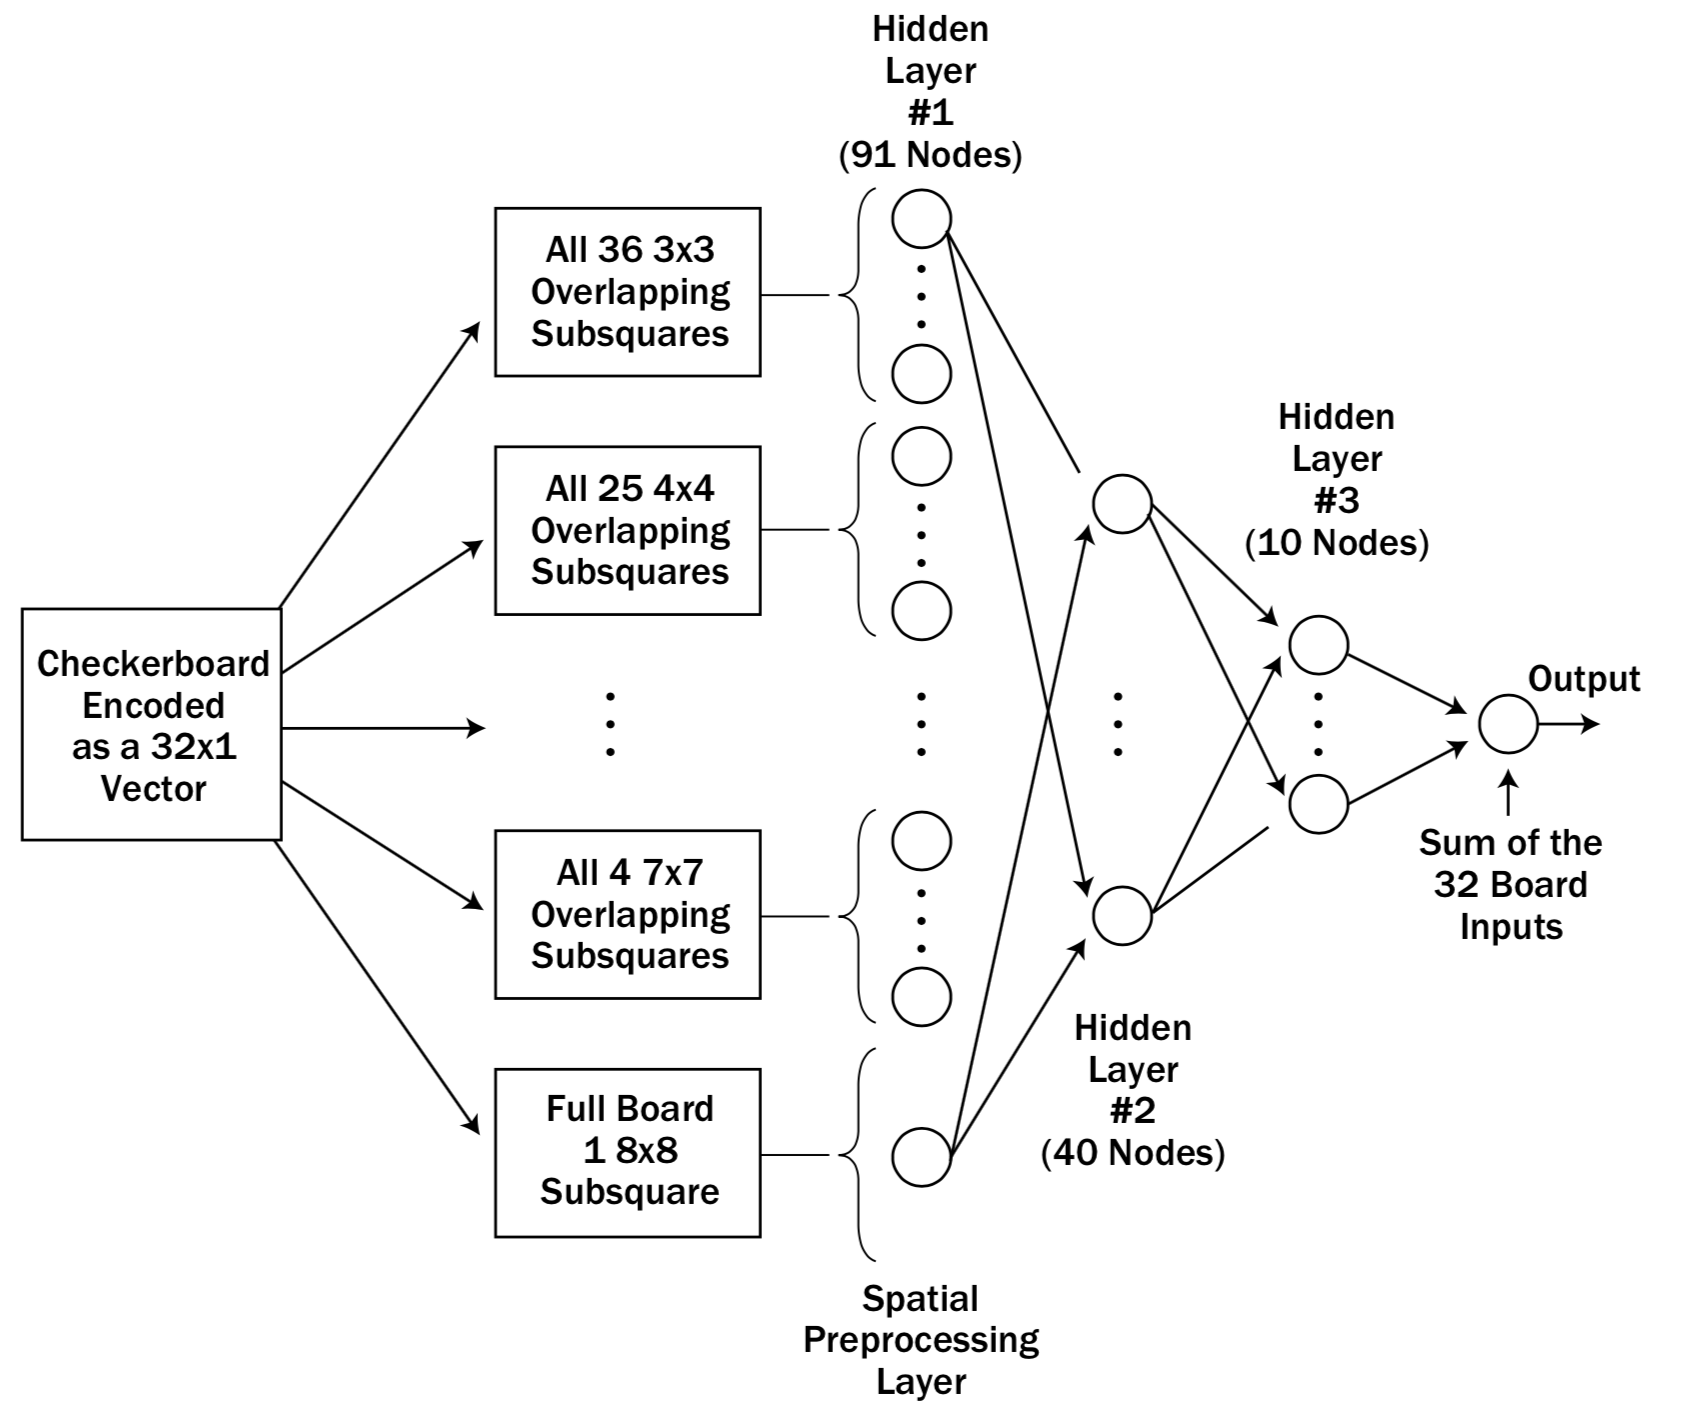
\includegraphics[width=100mm]{nnmodel.png}
    \caption{The chosen neural network model. Note that the checkboard is preprocessed. \label{overflow}}
\end{figure}

\subsubsection{MiniMax Decision Making}

The minimax algorithm revolves around the use of miniMax algorithm to determine the best move to make from a given position. The use of alpha-beta pruning will help to prune unnecessary calls.

\subsubsection{Tournament Method}

The tournament algorithm follows the following pseudocode in Algorithm 1.

% add pseudocode here
\begin{algorithm}
    \caption{My algorithm}\label{euclid}
    \begin{algorithmic}[1]
    \Procedure{MyProcedure}{}
    \State $\textit{stringlen} \gets \text{length of }\textit{string}$
    \State $i \gets \textit{patlen}$
    \BState \emph{top}:
    \If {$i > \textit{stringlen}$} \Return false
    \EndIf
    \State $j \gets \textit{patlen}$
    \BState \emph{loop}:
    \If {$\textit{string}(i) = \textit{path}(j)$}
    \State $j \gets j-1$.
    \State $i \gets i-1$.
    \State \textbf{goto} \emph{loop}.
    \State \textbf{close};
    \EndIf
    \State $i \gets i+\max(\textit{delta}_1(\textit{string}(i)),\textit{delta}_2(j))$.
    \State \textbf{goto} \emph{top}.
    \EndProcedure
    \end{algorithmic}
\end{algorithm}



\subsubsection{Genetic Algorithm}

The genetic algorithm 

\subsubsection{Population Generation}

The initial population will consist of randomly generated weights and biases of the neural network, with values from -1,1 inclusive. For a population size of 15, the next generation is created using this strategy:

The top five agents from the generation (at the end of the tournament round) are selected for crossover. They will continue to play in the next generation.
The next 8 players are generated in the following strategy:

The weights of the 1st and 2nd place agents are used as input to the crossover strategy and will generate 4 offsprings. Two are reciprocal crossover representations from the crossover, and the other two being directly mutated from the parents themselves. Another four children will be created using the same strategy, with the 2nd and 3rd agent's weights. 

The remaining two will be direct mutations of the 4th and 5th place agents.

\subsubsection{Coefficent Mutation}

Each weight of the neural network will be incremented by a random value that is created using the following formula, where $WeightP$ is the current weight, and $K$ represents the number of weights and biases in the neural network:

$$ WeightN = WeightP + \frac{1}{\sqrt{2 * \sqrt{K} }}$$

The weights, as explained earlier have a hard cap of [-1, 1].

\subsubsection{Crossover Strategy}

Two offsprings are created per a pair of parents, with each offspring being the reciprocal crossover of each other. The weights of both parents (now each treated as a 1D array of coefficents), are divided contingent on the number of weights and biases for a given layer. Each layer should be treated separately to reduce the potential dependency on a purely randomly generated neural network. For each set of weights in a given layer, the following algorithm represents the crossover process:

% add pseudocode here
\begin{algorithm}
    \caption{Crossover Strategy}\label{euclid}
    \begin{algorithmic}[1]
    \Procedure{crossover}{}
    \State $\textit{stringlen} \gets \text{length of }\textit{string}$
    \State $i \gets \textit{patlen}$
    \BState \emph{top}:
    \If {$i > \textit{stringlen}$} \Return false
    \EndIf
    \State $j \gets \textit{patlen}$
    \BState \emph{loop}:
    \If {$\textit{string}(i) = \textit{path}(j)$}
    \State $j \gets j-1$.
    \State $i \gets i-1$.
    \State \textbf{goto} \emph{loop}.
    \State \textbf{close};
    \EndIf
    \State $i \gets i+\max(\textit{delta}_1(\textit{string}(i)),\textit{delta}_2(j))$.
    \State \textbf{goto} \emph{top}.
    \EndProcedure
    \end{algorithmic}
\end{algorithm}

\subsection*{Testing and Evaluation}
The combined GANN (Genetic Algorithm/Neural Networks) are evaluated under competition style conditions. At each generation, each agent plays 5 games, with their opponment being from randomly chosen from the generation pool. Point scores are measured by {2,0,-1} where 2 is a win, 0 is a draw, and -1 is a loss. There is a hard cap of 50 moves, where the game is considered a draw if after the game hasn't ended after 50 moves from each player.

At the end of a given generation, we measure growth of performance using the champion of the generation. The score is calculated using the following formula, whatever it is.

Presently we will use the mean of means approach. When a new chapmion is generated, it is played against the previous 5 champions from earlier generations. 6 games are played for each previous champion, with 3 being as Black, and 3 being White. A mean score is calculated from those 6 games. The overall performance of the current chapmion is the mean of the 5 sets of games. A positive improvement is when the mean of means are greater than 0. 

Point Score for the champion games are measured by {1,0,-1} where a Win counts as 1 point and -1 for a loss. The weights are scaled differently to the regular tournament in order to accurately portray the difference between previous champions.

At the end of the generation run, the end player will be used to compete against human players on various online multiplayers checkers websites in order to determine an accurate ELO rating of the system.

% The algorithms described above will be evaluated under competition-style conditions. Each agent will play each game a number of times against every other agent to establish the winner. The starting player, number ofmoves and winning player. Each agent will be subject to the same time limit for choosing moves. Failure to return a move for any reason will result in an automatic loss. For each game, agents will play an equal number of rounds as first player. This will take into account any bias towards the player making the first move. For example, Checkers (Schaeffer et al, 2007) and Connect-Four (Allis, 1988) have both been solved, concluding that it is possible for the first player to force a win.

% A second round of testing will involve having each player choose moves for a predefined set of scenarios to analyse their behaviour and whether they consistently choose good moves (i.e. block an opponent from winning) or miss obvious winning/losing moves.

% There are two elements to the evaluation of the algorithms. First, I will examine the change in performance affected by changing the balance between the randomised monte-carol simulations and performing pre-computation to cut down the game tree. Second, I will attempt to create a rel- atively strong general game player using various enhancements that should be able to consistently beat the algorithms discussed above.

% ---

% I will evaluate my final system in two ways. First I will spend time comparing my system to other systems that are already available. I will select a number of such systems and compare them by a number of criteria that I will layout below which I believe cover the aims of my project. This will ensure that there is no one system that performs better than mine at my stated goals, even if they do outperform my solution in individual areas.
% The criteria that I use will be as follows:
% 1. Theabilityofthesystemtoclearlyrepresentthestateofandrelationshipsbetweenpeople
% 10
% 2. Theabilityofthesystemtorepresenttheinteractionsoverdifferentmodesbetweenpeople
% 3. The ability of the system to represent clustering of the people in the system based on interactions
% 4. The ability of the system to output quantitative data which can be used to draw useful conclusions regarding the nature of some aspect of the evolution of the model over time
% I will then judge this against the following systems:
% Vizster A project I have already discussed, designed to visualise connections between people in aFriendsternetwork. Availablefromhttp://homes.cs.washington.edu/jheer/projects/vizster/
% WolframAlpha Facebook Report An analysis of data gathered from your Facebook profile by the WolframAlpha website which includes a graphical representation of your friends and gives various indications of the roles friends play in the network. Available from https://www.wolframalpha.com/input/?i=facebook+report
% Gephi This is a tool developed for visualising graphs of all kinds of graph data in very config- urable ways. It also supports graphs that evolve over time and allows statistical analysis of graphs. Avaiable from http://gephi.github.io/
% Secondly I will measure the extent to which my system is able to solve a real-world problem. My prototyping will enable me to adapt my system to a wide variety of different problems in the field of social network research and so I will be able to look at existing solutions to these problems and compare my solution quantitatively to previous work.

% --------------------------------

% Presents the proposed solution(s)
% The design details should all be placed in this section
% Create a number of subsections, each focusing on one issue
% - Make it as clear as possible what you are planning to do
% - But not as a list of steps

% Writing skills (10%)
% • Clarity of presentation of ideas
% • Conformance to paper format
% standards as specified in
% Paper Template
% • Qualityofwriting(readability,
% grammar)
% • References

% Mark Scheme
% • Adequacy of the proposed solution
% • Specification and design
% • Identification of requirements
% • Description of tools used
% • Overview of architecture
% • Description of lifecycle

% This section presents the proposed solutions of the problems in detail. The design details should all be placed in this section. You may create a number of subsections, each focusing on one issue.

% This section should be up to 8 pages in length. The rest of this section shows the formats of subsections as well as some general formatting information.  You should also consult the Word template. 


\subsection{Figures and Tables}
In general, figures and tables should not appear before they are cited.  Place figure captions below the figures; place table titles above the tables.  If your figure has two parts, for example, include the labels ``(a)'' and ``(b)'' as part of the artwork.  Please verify that figures and tables you mention in the text actually exist.  make sure that all tables and figures are numbered as shown in Table \ref{units} and Figure 1.
%sort out your own preferred means of inserting figures

\begin{table}[htb]
\centering
\caption{UNITS FOR MAGNETIC PROPERTIES}
\vspace*{6pt}
\label{units}
\begin{tabular}{ccc}\hline\hline
Symbol & Quantity & Conversion from Gaussian \\ \hline
\end{tabular}
\end{table}

% ----------------

\subsection{References}

The list of cited references should appear at the end of the report, ordered alphabetically by the surnames of the first authors.  The default style for references cited in the main text is the  Harvard (author, date) format.  When citing a section in a book, please give the relevant page numbers, as in \cite[p293]{budgen}.  When citing, where there are either one or two authors, use the names, but if there are more than two, give the first one and use ``et al.'' as in  , except where this would be ambiguous, in which case use all author names.

You need to give all authors' names in each reference.  Do not use ``et al.'' unless there are more than five authors.  Papers that have not been published should be cited as ``unpublished'' \cite{euther}.  Papers that have been submitted or accepted for publication should be cited as ``submitted for publication'' as in \cite{futher} .  You can also cite using just the year when the author's name appears in the text, as in ``but according to Futher \citeyear{futher}, we \dots''.  Where an authors has more than one publication in a year, add `a', `b' etc. after the year.


\bibliography{projectpaper}


\end{document}